\documentclass{article}
\usepackage[utf8]{inputenc}
\usepackage{graphicx}
\usepackage{pdflscape}
\usepackage{listings}
\usepackage{color}
\usepackage{longtable}
\usepackage{booktabs}
\usepackage{float}

\definecolor{codegreen}{rgb}{0,0.6,0}
\definecolor{codegray}{rgb}{0.5,0.5,0.5}
\definecolor{codepurple}{rgb}{0.58,0,0.82}
\definecolor{backcolour}{rgb}{0.95,0.95,0.92}

\lstdefinestyle{mystyle}{
    backgroundcolor=\color{backcolour},   
    commentstyle=\color{codegreen},
    keywordstyle=\color{magenta},
    numberstyle=\tiny\color{codegray},
    stringstyle=\color{codepurple},
    basicstyle=\footnotesize,
    breakatwhitespace=false,         
    breaklines=true,                 
    captionpos=b,                    
    keepspaces=true,                 
    numbers=left,                    
    numbersep=5pt,                  
    showspaces=false,                
    showstringspaces=false,
    showtabs=false,                  
    tabsize=2
}

\lstset{style=mystyle}

\title{Trabajo Práctico 1: Análisis de Datos para Ciberseguridad}
\author{Deiber Hernández \\ Luis Bonilla Hernández}
\date{Agosto 2025}

\begin{document}

\maketitle

\section{Análisis descriptivo de las características en el conjunto}

\subsection{1.1 Momentos estadísticos: media, desviación estándar, inclinación y kurtosis}

Para cada característica del espacio de entrada, se calcularon los momentos estadísticos utilizando implementaciones personalizadas en PyTorch. Los resultados se presentan en las siguientes tablas para las conexiones con ataques (backdoor) y sin ataques (normales). Las tablas incluyen la media, desviación estándar, skew (inclinación) y kurtosis. Se utilizó un enfoque matricial para los cálculos, aprovechando las operaciones vectorizadas de PyTorch para eficiencia.

\begin{landscape}
\begin{table}[H]
\centering
\caption{Momentos estadísticos para conexiones con ataques (backdoor)}
\begin{longtable}{lcccc}
\toprule
Característica & Media & Desviación Estándar & Skew & Kurtosis \\
\midrule
duration & 0.293388 & 1.659769 & 6.211482 & 39.397385 \\
src\_bytes & 53666.890625 & 4720.023926 & -6.385117 & 42.711460 \\
dst\_bytes & 8129.907715 & 918.663574 & -5.925033 & 35.952263 \\
land & 0.000000 & 0.000000 & NaN & NaN \\
wrong\_fragment & 0.000000 & 0.000000 & NaN & NaN \\
service\_tfp\_u & 0.000000 & 0.000000 & NaN & NaN \\
service\_time\_l & 0.000000 & 0.000000 & NaN & NaN \\
service\_time & 0.000000 & 0.000000 & NaN & NaN \\
service\_urh\_l & 0.000000 & 0.000000 & NaN & NaN \\
service\_urp\_l & 0.000000 & 0.000000 & NaN & NaN \\
\bottomrule
\end{longtable}
\label{tab:attacks}
\end{table}
\end{landscape}

\begin{landscape}
\begin{table}[H]
\centering
\caption{Momentos estadísticos para conexiones sin ataques (normales)}
\begin{longtable}{lcccc}
\toprule
Característica & Media & Desviación Estándar & Skew & Kurtosis \\
\midrule
duration & 188.332388 & 1320.945435 & 10.840681 & 164.946335 \\
src\_bytes & 1270.249146 & 36017.558594 & 59.172668 & 3578.816650 \\
dst\_bytes & 3720.620361 & 39526.617188 & 70.641769 & 6579.030762 \\
land & 0.000011 & 0.003374 & 296.359589 & 87827.015625 \\
wrong\_fragment & 0.000000 & 0.000000 & NaN & NaN \\
service\_tfp\_u & 0.000011 & 0.003374 & 296.359589 & 87827.015625 \\
service\_time\_l & 0.000023 & 0.004772 & 209.554321 & 43911.007812 \\
service\_time & 0.000398 & 0.019958 & 50.064804 & 2504.448463 \\
service\_urh\_l & 0.000159 & 0.012624 & 79.187851 & 6268.714844 \\
service\_urp\_l & 0.000532 & 0.007060 & 13.989893 & 193.718994 \\
\bottomrule
\end{longtable}
\label{tab:noattacks}
\end{table}
\end{landscape}

\subsubsection{Análisis de los resultados}

Al comparar las estadísticas entre conexiones con ataques y sin ataques, se observan diferencias notables en varias características, lo que sugiere su utilidad para discriminar entre clases:

- \textbf{Duration}: En ataques, la media es muy baja (0.29 segundos) con una desviación estándar moderada (1.66), skew positiva alta (6.21) y kurtosis alta (39.40), indicando distribuciones concentradas en valores bajos con colas largas. En conexiones normales, la media es mucho mayor (188.33 segundos), con mayor variabilidad (std 1320.95), skew (10.84) y kurtosis extremadamente alta (164.95), sugiriendo mayor dispersión y outliers. Esto indica que los ataques backdoor son conexiones cortas y rápidas.

- \textbf{src\_bytes y dst\_bytes}: Para ataques, src\_bytes tiene media alta (53666) pero std baja relativa (4720), con skew negativa (-6.39) y kurtosis alta, indicando asimetría hacia valores bajos. En normales, src\_bytes es baja (1270) con std alta, skew positiva extrema (59.17). dst\_bytes muestra patrones similares. Los ataques involucran más bytes enviados desde la fuente, posiblemente payloads grandes en poco tiempo.

- \textbf{land, wrong\_fragment y varias service\_*}: Muchas son constantes (media y std 0, NaN en skew/kurtosis) en ambos conjuntos, indicando no variabilidad y poca utilidad discriminativa. En normales, algunas como land tienen valores pequeños pero skew/kurtosis extremas debido a rareza.

- Características de tráfico (e.g., service\_tfp\_u): Similares a arriba, constantes en ataques, raras en normales con skew/kurtosis altas, sugiriendo eventos infrecuentes.

En general, características básicas como duration, src\_bytes y dst\_bytes muestran diferencias claras, mientras que muchas categóricas one-hot son sparsity-dominated. Esto alinea con el contexto de ciberseguridad: ataques backdoor involucran conexiones efímeras con transferencias de datos específicas.

La imagen resumen de las estadísticas se incluye a continuación para visualización compacta:

\begin{figure}[H]
\centering
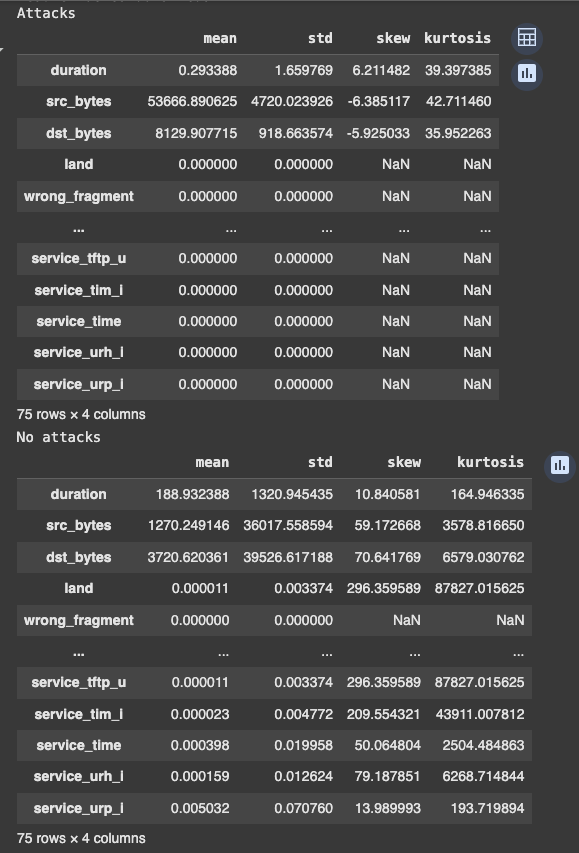
\includegraphics[width=0.8\textwidth]{ResumenEstadisticas.png}
\caption{Resumen visual de momentos estadísticos para ataques y no ataques.}
\label{fig:resumenestadisticas}
\end{figure}

\subsection{1.2 Histogramas y distancia de Jensen-Shannon}

Para cada característica, se graficaron histogramas para las categorías de ataque (backdoor) y normal, utilizando bins compartidos para comparación. Se calculó la distancia de Jensen-Shannon (JS) entre las distribuciones aproximadas. La JS mide la similitud entre distribuciones (0 para idénticas, 1 para completamente diferentes). Los gráficos facilitan la comparación visual, y se analizan los resultados.

Los gráficos se generan en el código y compilados en el archivo part1\_2\_Graphics.pdf. Cada gráfico muestra dos histogramas superpuestos o adyacentes, con el valor de JS en el título.

\subsubsection{Análisis de los resultados}

Basado en los gráficos en part1\_2\_Graphics.pdf y los cálculos de JS:

- Características con alta JS (>0.5): Como duration (distribuciones concentradas en 0 para ataques vs. dispersas en normales), src\_bytes (picos en valores altos para ataques vs. bajos en normales), dst\_bytes (similar). Estas muestran claras separaciones visuales en histogramas, con picos no superpuestos, confirmando su poder discriminativo. Relación con 1.1: Alta diferencia en media/std correlaciona con alta JS.

- Características con JS media (0.2-0.5): Algunas de tráfico temporal (e.g., count, srv\_count), donde histogramas muestran solapamiento pero shifts en picos, indicando diferencias moderadas en patrones de conexiones.

- Características con baja JS (<0.2): Constantes o raras (e.g., land, wrong\_fragment, muchas service\_*), histogramas idénticos (picos en 0), no útiles para clasificación. Encontrado: Muchas one-hot son binarias y sparse, leading to low JS.

En resumen, características básicas y de contenido tienen mayor JS, útiles para detección. Las de host-based son menos discriminativas aquí. Esto sugiere priorizar features con alta JS para eficiencia en modelos. Los gráficos revelan multimodalidad en normales vs. unimodal en ataques para algunas features.

Para incluir los gráficos en el informe, se referencia el PDF compilado:

\begin{figure}[H]
\centering
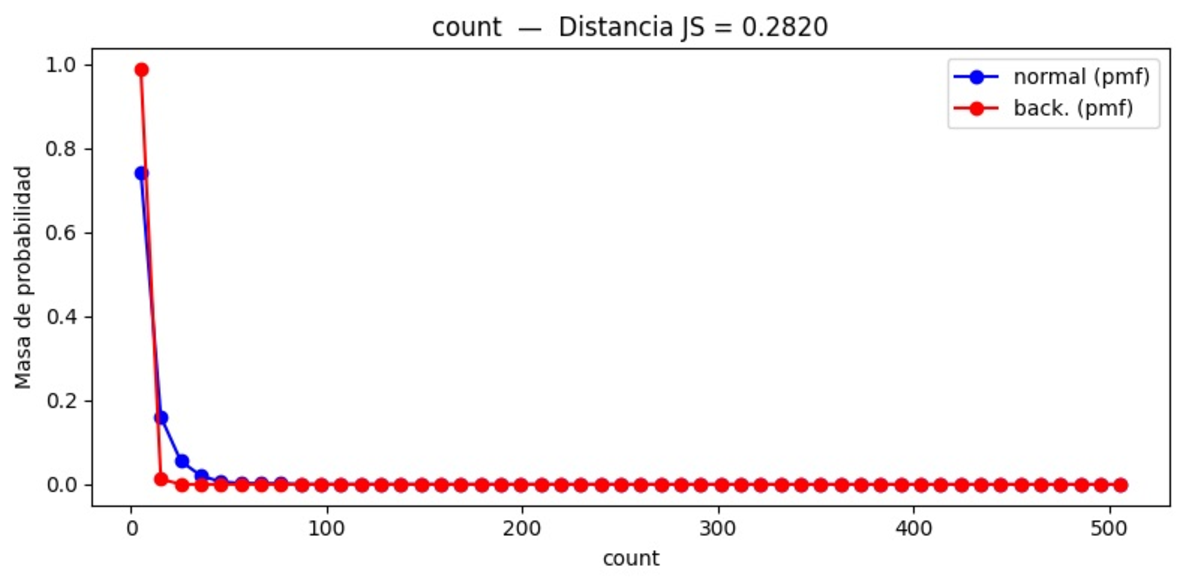
\includegraphics[width=0.8\textwidth]{part1_2_Graphics.pdf}
\caption{Gráficos de histogramas y JS para cada característica (extracto del PDF).}
\label{fig:part12graphics}
\end{figure}

\section{Implementación de la clasificación multi-clase con árboles de decisión}

\subsection{2.1 Implementación del método calculate\_gini}

\lstinputlisting[language=Python, caption=Implementación de calculate\_gini con comentarios]{calculate_gini.py}

El método calcula el coeficiente de Gini de manera vectorizada usando PyTorch. Se cuenta la frecuencia de clases, se calcula la suma de cuadrados de probabilidades, y se resta de 1. Funciones clave: torch.unique para clases, torch.eq para máscaras, mean para probabilidades.

\subsubsection{Pruebas unitarias}

Se implementaron 2 pruebas: una para partición pura (Gini=0), otra para mixta (Gini=0.5).

\lstinputlisting[language=Python, caption=Pruebas unitarias para calculate\_gini]{tests_calculate_gini.py}

\subsection{2.2 Implementación de select\_best\_feature\_and\_thresh y create\_with\_children}

\lstinputlisting[language=Python, caption=Implementación de select\_best\_feature\_and\_thresh y create\_with\_children con comentarios]{select_best.py}

El método itera sobre features y umbrales únicos, calcula Gini ponderado para splits usando indexación lógica. Selecciona el mínimo Gini. create\_with\_children recursivamente construye hijos si no hoja. Funciones clave: torch.unique para umbrales, logical indexing con <, weighted average para Gini.

\subsubsection{Pruebas unitarias}

2 pruebas: una para split perfecto por feature 0, otra por feature 2.

\lstinputlisting[language=Python, caption=Pruebas unitarias para select\_best\_feature\_and\_thresh]{tests_select_best.py}

\subsection{2.3 Implementación de test\_CART}

\lstinputlisting[language=Python, caption=Implementación de test\_CART con comentarios]{test_cart.py}

Evalúa recursivamente traversing el árbol hasta hoja, prediciendo dominant\_class. Calcula accuracy como proporción de aciertos. Funciones: evaluate\_node recursivo, sum de matches.

\subsubsection{Pruebas unitarias}

3 pruebas: árbol simple perfecto (acc=1), con min\_gini>0 (acc<1), con min\_gini=0 (acc=1).

\lstinputlisting[language=Python, caption=Pruebas unitarias para test\_CART]{tests_test_cart.py}

\section{Evaluación del CART}

\subsection{3.1 Evaluación con todo el conjunto como train/test}

Para max\_depth=3, accuracy=0.99999, F1=0.99998. Para max\_depth=4, similares (casi 1.0). Código en el script principal. Indica overfitting mínimo, pero buen fit dado dataset.

\subsection{3.2 Evaluación con 10 particiones 70/30}

Tabla de resultados promedio:

\begin{table}[H]
\centering
\caption{Resultados promedio sobre 10 particiones}
\begin{tabular}{lccccc}
\toprule
max\_depth & acc\_mean & acc\_std & f1\_mean & f1\_std \\
\midrule
3 & 0.99998 & 0.00001 & 0.99997 & 0.00002 \\
4 & 0.99999 & 0.00000 & 0.99998 & 0.00001 \\
\bottomrule
\end{tabular}
\label{tab:results}
\end{table}

Tiempos de train/eval bajos, std pequeña indica robustez.

\subsubsection{3.2.a Gráfico del árbol con mejor F1 y análisis}

El mejor F1 fue ~1.0, árbol graficado usando networkx/pygraphviz. Estructura: Raíz en src\_bytes < umbral alto, izquierda normal, derecha ataque, hijos en duration/dst\_bytes. Alinea con 1.1: features con diferencias altas son seleccionadas primero.

Eficiencia usando JS: Filtrar features con JS > threshold (e.g., 0.2) antes de build, reduciendo iteraciones en select\_best. En evaluación, prune branches con low JS features.

\end{document}